% This is samplepaper.tex, a sample chapter demonstrating the
% LLNCS macro package for Springer Computer Science proceedings;
% Version 2.21 of 2022/01/12
%
\documentclass[runningheads]{llncs}
%
\usepackage[T1]{fontenc}
% T1 fonts will be used to generate the final print and online PDFs,
% so please use T1 fonts in your manuscript whenever possible.
% Other font encondings may result in incorrect characters.
%
\usepackage{graphicx}
\usepackage{booktabs}
\usepackage{amsmath}
\usepackage{float}
% Used for displaying a sample figure. If possible, figure files should
% be included in EPS format.
%
% If you use the hyperref package, please uncomment the following two lines
% to display URLs in blue roman font according to Springer's eBook style:
%\usepackage{color}
%\renewcommand\UrlFont{\color{blue}\rmfamily}
%\urlstyle{rm}
%
\begin{document}
%
\title{Towards Robust Uzbek Neural Dependency Parsing}
%
%\titlerunning{Abbreviated paper title}
% If the paper title is too long for the running head, you can set
% an abbreviated paper title here
%
\author{Sanatbek Matlatipov\inst{1}\orcidID{0000-0002-6895-3436}}
%
\authorrunning{M. Sanatbek et al.}
% First names are abbreviated in the running head.
% If there are more than two authors, 'et al.' is used.
%
\institute{
National University of Uzbekistan named after Mirzo Ulugbek, Tashkent, Uzbekistan \\
\email{s.matlatipov@nuu.uz}
}
%
\maketitle              % typeset the header of the contribution
%
\begin{abstract}
This paper addresses the non-trivial tasks of morphosyntactic tagging and dependency parsing for Uzbek, a morphologically complex, resource-poor Turkic language with extensive agglutination and free constituent order. We train and evaluate a Stanza-based neural pipeline under two embedding regimes---static FastText vectors and the monolingual TahrirchiBERT contextual encoder---and across two data settings: the UzUDT treebank alone (684 sentences) and its combination with the UD\_Uzbek-UT treebank (1{,}184 sentences total). To align BERT subword outputs with UD word tokens, we apply a last-subword ``super-token'' fusion strategy. In the best configuration (TahrirchiBERT on merged data), the pipeline achieves 85.08 UPOS, 84.72 XPOS, and 71.09 UFeats tagging accuracy, together with 72.39 UAS and 63.81 LAS for dependency parsing, substantially outperforming the FastText-only baseline. Our experiments establish reproducible neural baselines for Uzbek UD parsing and quantify the impact of contextual embeddings and data augmentation via treebank merging.
\keywords{Uzbek \and Universal Dependencies \and morphosyntactic tagging \and neural dependency parsing \and contextual embeddings \and TahrirchiBERT}
\end{abstract}

%
%
%
\section{Introduction}

The state of Natural Language Processing (NLP) in today's world is characterized by a large gap between highly resourced languages such as English, Chinese, and Spanish, and the remainder of the languages in the world that are still under-resourced in terms of their technological advancement\cite{blasi-etal-2022-systematic}. The challenge gets accentuated in cases where languages possess complex morphological structures, making their syntactic and semantic expression difficult to formalize through standard models that are designed for analytical types of languages. Uzbek is one such language that belongs to the Turkic family of languages, is considered to be a language of significance in terms of population\cite{KROUGLOV2017173}\footnote{\url{https://www.sciencedirect.com/topics/social-sciences/uzbek}}, but is a low-resource language since it serves as the national language of Uzbekistan and has a population of over 37 million in Central Asia\footnote{\url{https://www.worldometers.info/world-population/uzbekistan-population/}}.

The development of efficient parsing tools for Uzbek is very important and can be considered a foundation for implementing efficient artificial intelligence systems in this region. Parsing sentences syntactically, and more specifically, parsing them using dependencies, has been recognized as a foundation for a variety of applications in Natural Language Processing, such as Machine Translation, Sentiment Analysis, Named Entities Recognition, and Information Extraction applications, to name a few. Being a morphologically agglutinative language, having a relatively free Subject-Object-Verb (SOV) order\cite{nilufar-abdurakhmon} \cite{linguistic-feat}, and being a rather complex language in terms of syntactic dependencies, for a language such as Uzbek, syntactic dependencies\cite{11206779} are crucial for improving disambiguations of meanings in sentences. Unlike in English, where precedence determines grammatical relations, in Uzbek, a complex system based on cases that are prefixed or suffixed to members of a noun phrase or to emphasize a verb, makes parsing more challenging, as a parser should be able to move beyond token position to identify deeper structures in texts for their interpretation [4].

Dependency parsing underpins many higher-level NLP capabilities: it provides a compact, interpretable representation of grammatical relations that supports information extraction, machine translation, question answering, and knowledge graph construction. Although some progress has been achieved in multilingual parsing tasks, the current state of parsing research for the Uzbek language remains unsatisfactory due to a lack of high-quality parsing benchmarks and pretrained models. There are two main reasons for this state of affairs. Firstly, there is a lack of annotated data, and secondly, the Uzbek language is agglutinative, and productive suffixation, rich case marking, flexible word order, sparsity, and function words with multiple functions are a challenge for any parsing algorithm.

The goal of this work is to make Uzbek morphosyntactic analysis---jointly modeling POS/morphological features and dependency structure in the Universal Dependencies (UD) framework---more practical and robust for real NLP use. Using two publicly available Uzbek UD treebanks---UzUDT (684 sentences, authored by the present author) and UD\_Uzbek-UT (500 sentences)---we develop and evaluate reproducible neural baselines for Uzbek tagging and dependency parsing in a Stanza-style pipeline\cite{Qi2020-zr}. We compare two embedding regimes: static FastText word vectors and the monolingual TahrirchiBERT contextual encoder, and evaluate each on two data settings (UzUDT alone and a merged corpus combining both treebanks). To bridge the mismatch between BERT subword tokenization and UD word tokens, we employ a fixed last-subword ``super-token'' fusion strategy\cite{Ho2021-cc}, \cite{hopton-etal-2025-functional}. The expected outcomes are (i) standardized UD evaluation results and training recipes that can be reliably replicated, (ii) a quantitative assessment of the impact of contextual embeddings and cross-treebank data augmentation in a low-resource setting, and (iii) diagnostic analyses that explain current failure modes and guide future model improvements.

\paragraph{Contributions.}
This paper focuses on robust morphosyntactic tagging and dependency parsing for Uzbek, utilizing publicly available data from two Uzbek UD treebanks. Although details about UzUDT construction have been discussed in another submission, this paper makes the following contributions:
\begin{itemize}
    \item \textbf{Reproducible Uzbek UD baselines.} We train and evaluate neural baselines for Uzbek morphosyntactic tagging (UPOS/XPOS/UFeats) and dependency parsing (UAS/LAS) under a standard UD evaluation setting, comparing static and contextual embedding regimes.\footnote{Training and evaluation code: \url{https://github.com/SanatbekMatlatipov/robust-parsing-uzbek}. Pretrained checkpoints/models: \url{https://huggingface.co/Sanatbek/uzudt}.}
    \item \textbf{Contextualized token representations.} We integrate the monolingual TahrirchiBERT encoder into the Stanza POS tagger and dependency parser with UD-aligned subword-to-word pooling (``super-token'' fusion via last-subword selection) to obtain word-level contextual representations suitable for UD parsing.
    \item \textbf{Cross-treebank data augmentation.} We evaluate the effect of merging two complementary Uzbek UD treebanks---UzUDT and UD\_Uzbek-UT---demonstrating that the combined data substantially improves parsing accuracy.
\end{itemize}



\section{Related Work}
\paragraph{Universal Dependencies.}
 UD treats words as syntactic units with morphological properties that enter into grammatical relations, and it emphasises transparent mapping from surface forms to tokens.  This uniform representation addresses earlier difficulties in comparing empirical results across languages and enables cross-lingual structure transfer. \cite{de-marneffe-etal-2021-universal} present a cross-linguistic perspective on the UD framework, reviewing its application to over one hundred languages.  They highlight how UD's universal POS tags and feature schema facilitate multilingual evaluation and typological research.  The UD guidelines (Version 2\footnote{\url{https://universaldependencies.org/guidelines.html}}) also document how tokenization, multiword expressions, lemmas, UPOS/XPOS tags, morphological features and dependency relations should be annotated;

\paragraph{Parsing in Turkic and other agglutinative languages.}
Agglutinative languages such as Turkish, Uzbek and other Turkic languages pose unique challenges for dependency parsing.  Rich morphology leads to long word-internal suffix chains, free word order complicates attachment, and function words often have multiple grammatical functions\cite{MURZINTCEV2026100195}.  Previous work on Turkish shows that morphology aware representations improve parsing accuracy; e.g., \cite{eryigit-etal-2008-dependency} introduce rule-based and neural models that incorporate morphological segmentation and show gains over purely lexical baselines.  Research on Kazakh, Uyghur and Tatar UD treebanks reports similar findings: parsers benefit from subword-level features and language-specific heuristics to resolve case-driven ambiguities\cite{Marsan_undated-hp}.  \cite{noauthor_2018-qq} discuss the difficulties of adapting UD guidelines to Turkish multi-word expressions and clitic constructions, emphasising the need for consistent morphological analysis.  These studies motivate our approach of combining neural encoders with morphology-aware subword representations.

\paragraph{Uzbek resources.}
Uzbek remains comparatively under-resourced for UD-style morphosyntactic analysis and dependency parsing. There are currently two available UD treebanks. An initial UD-compliant treebank (UD\_Uzbek-UT), containing 500 sentences from news and fiction genres, was released in 2024 with semi-automatic annotation and full manual correction~\cite{akhundjanova-talamo-2025-universal}. In this work, we additionally use the Uzbek UD treebank \emph{UzUDT} (684 sentences, 7{,}800 tokens), a manually annotated resource covering literature and academic text. The design rationale, annotation methodology, and quality assurance procedures for UzUDT are described in a companion paper submitted to the same venue by the present author~\cite{matlatipov2025goldudt}. By combining both treebanks, we obtain a merged corpus of 1{,}184 sentences, which we use to evaluate the effect of data augmentation on parsing quality.

\paragraph{Neural pipelines and contextual models.}
Fully neural multilingual NLP pipelines have seen rapid progress in recent years.  Stanza~\cite{Qi2020-zr} introduced a language-agnostic pipeline for tokenization, multi-word token expansion, lemmatization, POS morphological tagging, dependency parsing and named entity recognition.   Stanza's design is fully neural and processes raw text end-to-end.  The biaffine graph-based parser of \cite{DBLP:conf/iclr/DozatM17} remains a strong baseline; it uses MLP projections and biaffine classifiers for arcs and relations, achieving high accuracies on CoNLL-U corpora.  \cite{kondratyuk-straka-2019-75} further demonstrate that a single multilingual model (UDify) can parse 75 languages via joint multitask learning.   For Uzbek specifically, \cite{kuriyozov-etal-2024-bertbek} introduce \textit{BERTbek}, a transformer-based model pretrained on Uzbek news text, and show that monolingual contextual embeddings outperform mBERT on downstream tasks. In this work, we adopt TahrirchiBERT (\texttt{tahrirchi/tahrirchi-bert-base}), a monolingual Uzbek BERT model with broader domain coverage, which we integrate directly into Stanza's POS tagger and dependency parser modules.

\paragraph{Morphological analysis.}
Rule-based morphological analysers are valuable in agglutinative languages to supplement neural models. Apertium is a well-known open-source platform for rule-based machine translation that includes finite-state morphological analysers for numerous languages~\cite{Forcada2011}, including Uzbek~\cite{Salaev2024, 2301.12711, MURZINTCEV2026100195}. While morphological normalization can potentially reduce lexical sparsity, our experiments showed that the UD treebanks already contain consistent lemma annotations and that Apertium-based preprocessing produces zero form changes on Latin-NFC-normalized data. Consequently, we do not employ rule-based morphological normalization in our pipeline and instead rely entirely on the neural encoder's capacity to handle morphological variation through contextual subword representations.

\section{Datasets}
\label{sec:datasets}

\subsection{UD\_Uzbek-UzUDT}
\label{subsec:uzudt}
We use the publicly available Uzbek Universal Dependencies treebank UzUDT, released as a 3-star repository in the UD ecosystem.\footnote{UD repository: \url{https://github.com/UniversalDependencies/UD_Uzbek-UzUDT/tree/master}.\\
\url{https://universaldependencies.org/treebanks/uz_uzudt/index.html}.}
This treebank contains 684 sentences and approximately 7{,}800 tokens drawn from Uzbek literature and academic writing, annotated in UD v2 format with lemmas, UPOS/XPOS tags, morphological features, and dependency relations. Sentences were annotated by six annotators (four linguists and two NLP engineers) with full adjudication on the INCEpTION platform~\cite{matlatipov2025goldudt}.

\subsection{UD\_Uzbek-UT}
\label{subsec:ut}
The second treebank is UD\_Uzbek-UT, introduced by \cite{akhundjanova-talamo-2025-universal}. It contains 500 sentences (approximately 5{,}850 tokens) from news articles (250 sentences) and fiction (250 sentences). Annotation was semi-automatic with full manual correction. Because the original release contained only a single test file with all 500 sentences, we split the data sequentially into train/dev/test using the same proportions as UzUDT (approximately 66\%/7\%/27\%).

\subsection{Data settings and splits}
\label{subsec:splits}
Neither treebank originally provided a development set. We created dev splits by applying consistent $\approx$66/7/27 proportions across both corpora. This yields two data settings, summarized in Table~\ref{tab:data_splits}:

\begin{enumerate}
    \item \textbf{UzUDT only.} The baseline setting uses only UzUDT (684 sentences).
    \item \textbf{UzUDT + UT merged.} The combined setting merges both treebanks to form a larger corpus (1{,}184 sentences), testing whether cross-treebank data augmentation improves parsing accuracy.
\end{enumerate}

\begin{table}[t]
\centering
\small
\begin{tabular*}{\textwidth}{@{\extracolsep{\fill}}llrrrr@{}}
\toprule
\textbf{Setting} & \textbf{Split} & \textbf{Sentences} & \textbf{Sent.\,\%} & \textbf{Source} \\
\midrule
\multirow{4}{*}{UzUDT only} & Train & 451 & 65.9 & UzUDT \\
 & Dev & 45 & 6.6 & UzUDT \\
 & Test & 188 & 27.5 & UzUDT \\
 & \textit{Total} & \textit{684} & & \\
\midrule
\multirow{4}{*}{UzUDT + UT} & Train & 781 & 65.9 & UzUDT + UT \\
 & Dev & 78 & 6.6 & UzUDT + UT \\
 & Test & 325 & 27.4 & UzUDT + UT \\
 & \textit{Total} & \textit{1{,}184} & & \\
\bottomrule
\end{tabular*}
\caption{Data splits for the two evaluation settings. The merged setting concatenates UzUDT (451/45/188) with UD\_Uzbek-UT (330/33/137) train/dev/test files. Percentages are computed over each setting's total.}
\label{tab:data_splits}
\end{table}

Note that the UD\_Uzbek-UT corpus is ordered with news sentences first (1--250) and fiction second (251--500); consequently, the sequential train/dev/test split means training is predominantly news-genre while the test set is predominantly fiction, producing a realistic cross-genre evaluation scenario.

\section{Methodology}
\label{sec:methodology}

Figure~\ref{fig:uzbek_baseline_architecture} presents the end-to-end baseline architecture. Starting with an input sentence expressed as a sequence of Uzbek words, the architecture entails (i) UD-compliant tokenization and text normalization, (ii) contextualized embedding with a monolingual pretrained Transformer (TahrirchiBERT), (iii) word-level alignment of subword vectors through ``super-token'' fusion, and (iv) Universal Dependencies (UD) morphosyntactic tagging and dependency parsing. The architecture is specifically designed to address two Uzbek-specific challenges: (a) data scarcity due to agglutinative morphotactics, and (b) subword--UD token misalignment in Transformers. To mitigate these challenges, the pipeline combines deep contextual embedding with a fixed subword-to-UD token mapping.

\begin{figure}[t]
  \centering
    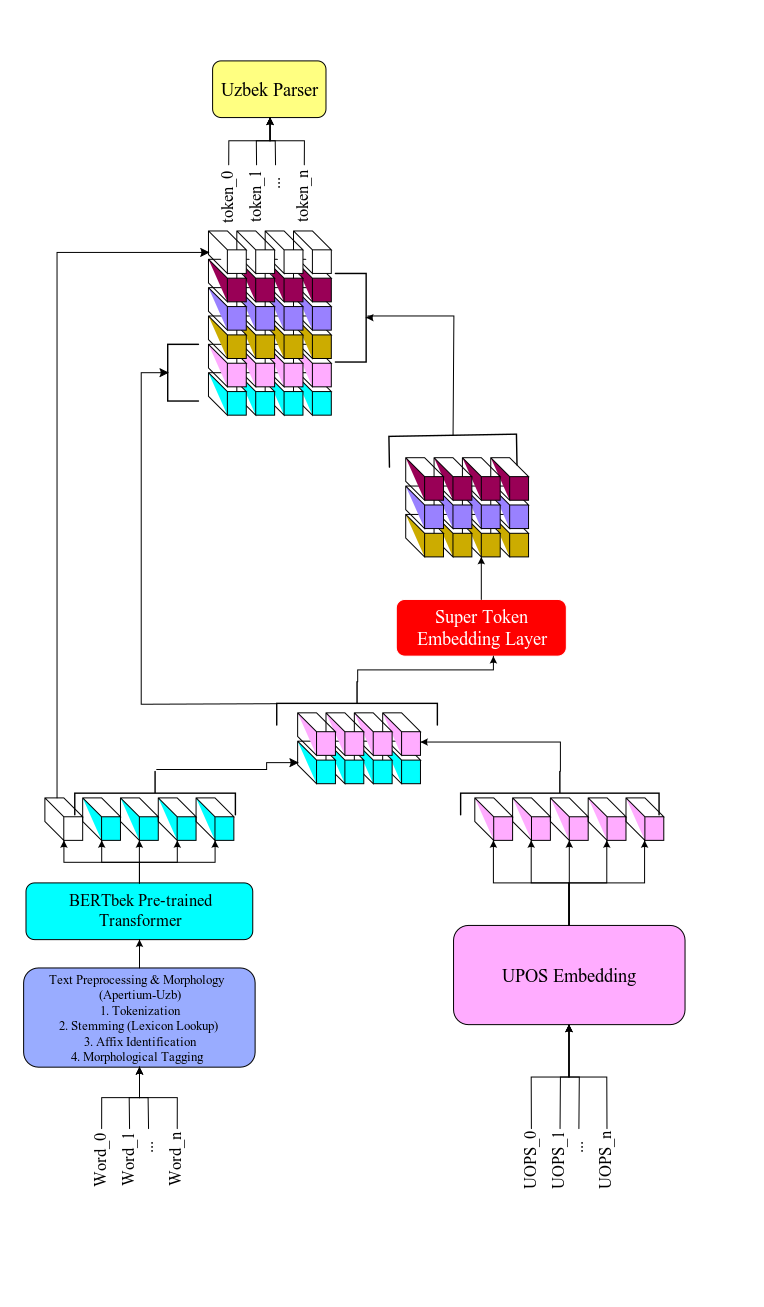
\includegraphics[width=0.75\linewidth]{baseline_architecture.png}
  \caption{Baseline Uzbek UD parsing framework. Uzbek tokens are encoded by TahrirchiBERT (or represented with static FastText vectors in the baseline configuration). Subword representations are aggregated into word-level vectors (``super-token'' fusion via last-subword selection) aligned to UD tokens. The parser consumes the fused word representations together with UPOS embeddings (from the tagging module) to predict dependency arcs and relations.}
  \label{fig:uzbek_baseline_architecture}
\end{figure}

\subsection{Preprocessing}
\label{subsec:preprocessing}
Let a sentence be $S=(w_1,\dots,w_n)$, where $w_i$ are UD word tokens. We apply:
\begin{enumerate}
    \item \textbf{Text normalization and UD-compliant tokenization.} Unicode normalization (NFC) and strict satisfaction of UD formatting constraints are used to provide stable token boundaries and evaluation compatibility.
    \item \textbf{Subword tokenization for TahrirchiBERT.} TahrirchiBERT operates on subword units, meaning each word $w_i$ is split into a subsequence of WordPiece symbols. The mapping of UD tokens to their subword segments is maintained for the subsequent fusion stage.
\end{enumerate}

\begin{figure}[H]
  \centering
  \includegraphics[width=0.85\linewidth]{verb-noun.png}
  \caption{Illustration of Uzbek morphotactics for verbs (top) and nouns (bottom): from a lexical stem, suffix sequences encode grammatical categories such as tense/voice/person (verbs) and number/possession/case (nouns).}
  \label{fig:uzbek_morphotactics}
\end{figure}

Figure~\ref{fig:uzbek_morphotactics} illustrates the common suffix chaining rules for verbs and nouns in Uzbek. These agglutinative morphotactics are a key source of data sparsity and motivate the use of subword-level contextual representations. Because the UD treebanks already contain consistent lemma annotations, we rely on the neural encoder's contextual representations rather than external rule-based morphological normalization.

\subsection{Token representations and ``super-token'' fusion}
\label{subsec:repr}
For each Universal Dependencies (UD) token $w_i$, a word-level representation is constructed by combining lexical, subword, and contextual information. In the TahrirchiBERT configuration, the contextual subword representations are denoted $\mathbf{z}_{i,1},\dots,\mathbf{z}_{i,m_i}$, referring to the $m_i$ subwords corresponding to $w_i$. Because UD evaluation is performed at the word level, an aggregation function is needed to produce a single word-level vector from the subword outputs.

We adopt a \emph{last-subword selection} strategy as the ``super-token'' fusion mechanism:
\begin{equation}
\mathbf{e}_{\text{ctx}}(w_i) = \mathbf{z}_{i,m_i},
\end{equation}
where $\mathbf{z}_{i,m_i}$ is the hidden state of the last subword in the span corresponding to $w_i$. This choice is motivated by the observation that in agglutinative languages such as Uzbek, the final subword of a word often encodes suffix-level grammatical information, making it a natural alignment point for UD-level morphosyntactic prediction.\footnote{We use a fixed fusion rule for all experiments to keep the baseline reproducible. Alternative strategies (mean pooling, first subword) are left for future work.}

In the FastText baseline configuration (without BERT), $\mathbf{e}_{\text{ctx}}(w_i)$ is not used and the model relies solely on pretrained static word vectors and character-level features.

We then form the final token vector:
\begin{equation}
\mathbf{x}_i =
\Big[
\mathbf{e}_{\text{word}}(w_i);\
\mathbf{e}_{\text{char}}(w_i);\
\mathbf{e}_{\text{upos}}(\hat{p}_i);\
\mathbf{e}_{\text{ctx}}(w_i)
\Big],
\end{equation}
where $\mathbf{e}_{\text{word}}$ and $\mathbf{e}_{\text{char}}$ are standard word- and character-level embeddings, $\mathbf{e}_{\text{ctx}}$ is the TahrirchiBERT-derived contextual embedding defined above (or absent in the FastText-only configuration), and $\mathbf{e}_{\text{upos}}(\hat{p}_i)$ is the UPOS embedding derived from the tagger output $\hat{p}_i$ (see below).

\subsection{Morphosyntactic tagging}
\label{subsec:tagging}
We train a neural morphosyntactic tagger to predict UPOS, XPOS, and UD morphological features. The tagger is implemented as a BiLSTM over the token sequence $\mathbf{x}_1,\dots,\mathbf{x}_n$:
\begin{equation}
\mathbf{h}_1,\dots,\mathbf{h}_n = \textsc{BiLSTM}(\mathbf{x}_1,\dots,\mathbf{x}_n).
\end{equation}
For each tagging task $t \in \{\textsc{UPOS}, \textsc{XPOS}, \textsc{UFeats}\}$ we compute:
\begin{equation}
p(y^t_i \mid S) = \text{softmax}(\mathbf{W}_t\mathbf{h}_i + \mathbf{b}_t).
\end{equation}
The tagging loss is the sum of cross-entropies across tasks:
\begin{equation}
\mathcal{L}_{\text{tag}} = \sum_{t}\sum_{i=1}^{n} -\log p(y^t_i \mid S).
\end{equation}

\paragraph{Avoiding oracle information.}
To prevent leakage of gold tags at inference time, UPOS embeddings used by the parser are computed from the \emph{predicted} UPOS labels $\hat{p}_i$ produced by the tagger. During training, we may optionally use gold UPOS embeddings for stabilization (teacher forcing), but all reported results are produced under the standard pipeline setting where predictions are used at test time.

\subsection{Dependency parsing}
\label{subsec:parsing}
Given encoder outputs $\mathbf{h}_i$, we employ a biaffine graph-based dependency parser~\cite{DBLP:conf/iclr/DozatM17}. We project tokens into head and dependent spaces:
\begin{equation}
\mathbf{r}^{\text{head}}_i=\text{MLP}_{\text{head}}(\mathbf{h}_i),\quad
\mathbf{r}^{\text{dep}}_j=\text{MLP}_{\text{dep}}(\mathbf{h}_j).
\end{equation}
Arc scores between candidate head $i$ and dependent $j$ are:
\begin{equation}
s^{\text{arc}}_{i,j} = (\mathbf{r}^{\text{head}}_i)^\top \mathbf{U}_{\text{arc}}\, \mathbf{r}^{\text{dep}}_j
+ \mathbf{w}_{\text{arc}}^\top [\mathbf{r}^{\text{head}}_i;\mathbf{r}^{\text{dep}}_j] + b_{\text{arc}}.
\end{equation}
Relation scores are computed analogously with label-specific parameters. The parsing loss combines arc and relation components:
\begin{equation}
\mathcal{L}_{\text{parse}} = \mathcal{L}_{\text{arc}} + \mathcal{L}_{\text{rel}},
\end{equation}
and the overall objective jointly trains tagging and parsing:
\begin{equation}
\mathcal{L} = \mathcal{L}_{\text{tag}} + \lambda\,\mathcal{L}_{\text{parse}}.
\end{equation}

\subsection{Evaluation}
\label{subsec:evaluation}
We evaluate morphosyntactic taggers on UPOS accuracy, XPOS accuracy, UD feature accuracy (UFeats), and joint tag accuracy (AllTags). For dependency parsing, we report UAS (unlabeled attachment score) and LAS (labeled attachment score), computed using the standard UD evaluation script. All evaluations use the predefined test splits described in Section~\ref{subsec:splits}.

\section{Experiments and Results}
\label{sec:experiments}

\subsection{Experiment matrix}
\label{subsec:matrix}
We define two embedding configurations, each evaluated on two data settings, yielding four experimental runs (Table~\ref{tab:matrix}):

\begin{table}[t]
\centering
\small
\begin{tabular*}{\textwidth}{@{\extracolsep{\fill}}llllp{5cm}@{}}
\toprule
\textbf{Run} & \textbf{Embeddings} & \textbf{Data} & \textbf{Fusion} & \textbf{Description} \\
\midrule
E1.1 & FastText & UzUDT & --- & Static embeddings, UzUDT only \\
E1.2 & FastText & UzUDT+UT & --- & Static embeddings, merged data \\
E2.1 & TahrirchiBERT & UzUDT & Last-sub & Contextual, UzUDT only \\
E2.2 & TahrirchiBERT & UzUDT+UT & Last-sub & Contextual, merged data \\
\bottomrule
\end{tabular*}
\caption{Experiment matrix. ``Last-sub'' denotes last-subword selection for super-token fusion. FastText experiments use \texttt{cc.uz.300.vec} (300-dim). TahrirchiBERT experiments use \texttt{tahrirchi/tahrirchi-bert-base} (768-dim).}
\label{tab:matrix}
\end{table}

For each run, we train a POS tagger followed by a dependency parser, then evaluate on the corresponding test set.

\subsection{Training setup}
\label{subsec:training_setup}
All models are trained within the Stanza framework using the default optimization settings. Table~\ref{tab:hyperparams} summarizes the architecture and optimization hyperparameters.

\begin{table}[t]
\centering
\small
\begin{tabular}{p{0.55\linewidth}p{0.35\linewidth}}
\toprule
\textbf{Hyperparameter} & \textbf{Value} \\
\midrule
\multicolumn{2}{l}{\textit{Model / architecture}} \\
\midrule
No.\ of parser hidden layers (MLP depth) & 1 (arc MLP) + 1 (rel MLP) \\
Parser hidden dimension (MLP) & 500 \\
UPOS embedding dimension & 50 \\
Super-token fusion (subword $\to$ word) & last-subword selection \\
Super-token embedding dimension & 768 (TahrirchiBERT) \\
Dropout & 0.33 \\
\midrule
\multicolumn{2}{l}{\textit{Optimization / scheduling}} \\
\midrule
Optimizer & Adam \\
Adam $\beta$ & (0.9, 0.999) \\
Learning rate & $3 \times 10^{-3}$ \\
Batch size & 5{,}000 tokens \\
Max training steps & 50{,}000 (early stopping on dev) \\
\bottomrule
\end{tabular}
\caption{Training setup and hyperparameters for the Uzbek baseline pipeline. ``Super-token'' refers to the subword-to-word aggregation step aligning TahrirchiBERT subword outputs to UD word tokens. In FastText experiments, the contextual embedding component is absent.}
\label{tab:hyperparams}
\end{table}

\subsection{Training and evaluation protocol}
We train a Stanza-style pipeline consisting of (i) a neural morphosyntactic tagger predicting UPOS, XPOS, and UD morphological features, and (ii) a biaffine graph-based dependency parser. Preprocessing follows Section~\ref{subsec:preprocessing} (UD-compliant tokenization and text normalization). In the TahrirchiBERT configuration, we apply a fixed last-subword ``super-token'' fusion strategy to aggregate subword vectors into UD-aligned word-level representations (Section~\ref{subsec:repr}). UPOS embeddings consumed by the parser are derived from predicted UPOS tags to avoid oracle information at inference time.

\subsection{Morphosyntactic tagging results}
Table~\ref{tab:tagging} summarizes tagging performance across all four experimental configurations. The best results are achieved by E2.2 (TahrirchiBERT on merged data): 85.08 UPOS, 84.72 XPOS, and 71.09 UFeats. TahrirchiBERT consistently outperforms the FastText baseline on UPOS, with the gain amplified on the merged dataset (+4.82 points). Merging treebanks provides modest improvements in UPOS and XPOS across both embedding regimes, and a substantial gain in UFeats for the TahrirchiBERT configuration (+5.72 points).

\begin{table}[H]
\centering
\small
\begin{tabular*}{\textwidth}{@{\extracolsep{\fill}}llrrrr@{}}
\toprule
\textbf{Run} & \textbf{Configuration} & \textbf{UPOS} & \textbf{XPOS} & \textbf{UFeats} \\
\midrule
E1.1 & FastText, UzUDT & 79.19 & 79.81 & 66.61 \\
E1.2 & FastText, UzUDT+UT & 80.26 & 83.20 & 66.98 \\
E2.1 & TahrirchiBERT, UzUDT & 82.45 & 80.90 & 65.37 \\
E2.2 & TahrirchiBERT, UzUDT+UT & \textbf{85.08} & \textbf{84.72} & \textbf{71.09} \\
\bottomrule
\end{tabular*}
\caption{Morphosyntactic tagging results on the test sets (accuracy, \%). Bold denotes the best result in each column.}
\label{tab:tagging}
\end{table}

\subsection{Dependency parsing results}
Table~\ref{tab:parsing} reports parsing performance. The best system (E2.2) achieves 72.39 UAS and 63.81 LAS. Notably, the most dramatic improvements come from treebank merging rather than from the embedding change: LAS jumps by +11.16 points for FastText (E1.1$\to$E1.2) and by +9.62 points for TahrirchiBERT (E2.1$\to$E2.2). TahrirchiBERT provides a consistent UAS improvement over FastText and a modest LAS gain on merged data (+1.41 points).

\begin{table}[H]
\centering
\small
\begin{tabular*}{\textwidth}{@{\extracolsep{\fill}}llrr@{}}
\toprule
\textbf{Run} & \textbf{Configuration} & \textbf{UAS} & \textbf{LAS} \\
\midrule
E1.1 & FastText, UzUDT & 69.57 & 51.24 \\
E1.2 & FastText, UzUDT+UT & 72.27 & 62.40 \\
E2.1 & TahrirchiBERT, UzUDT & 72.05 & 54.19 \\
E2.2 & TahrirchiBERT, UzUDT+UT & \textbf{72.39} & \textbf{63.81} \\
\bottomrule
\end{tabular*}
\caption{Dependency parsing results on the test sets (accuracy, \%). Bold denotes the best result in each column.}
\label{tab:parsing}
\end{table}

\subsection{Dependency-relation distribution and corpus diagnostics}
\label{subsec:deprel_dist}
\begin{figure}[H]
    \centering
    \includegraphics[width=0.72\linewidth]{top-20-dep-relations}
    \caption{Top 20 dependency relations in UzUDT. The chart highlights the skewed distribution of relations, with \texttt{punct} and frequent grammatical relations such as \texttt{obl}, \texttt{nsubj}, and \texttt{root} accounting for a large portion of the annotations.}
    \label{fig:deprel_top20}
\end{figure}
To contextualize model behavior, Figure~\ref{fig:deprel_top20} shows the frequency of the top 20 dependency relations in UzUDT. The distribution is highly skewed: \texttt{punct} dominates, followed by frequent core and oblique relations such as \texttt{obl}, \texttt{nsubj}, and \texttt{root}. A second tier includes common modifiers and clause-level relations (\texttt{amod}, \texttt{advcl}, \texttt{obj}) as well as coordination and nominal modification (\texttt{compound}, \texttt{nmod}, \texttt{conj}).

\section{Discussion}
\label{sec:discussion}
Our experiments investigate the interplay between embedding quality and training data quantity for Uzbek morphosyntactic tagging and dependency parsing in low-resource settings. We organize the discussion around three themes: the effect of contextual embeddings, the impact of treebank merging, and the persistent challenges of Uzbek.

\subsection{Effect of contextual embeddings}
\label{subsec:disc_bert}
Replacing static FastText embeddings with TahrirchiBERT yields consistent gains on UPOS tagging: +3.26 points on UzUDT alone (79.19$\to$82.45) and +4.82 points on merged data (80.26$\to$85.08). The contextual encoder helps the model generalize across morphological variants, effectively reducing the surface-form sparsity that limits static embeddings. However, the improvement on LAS is more modest: +2.95 on UzUDT (51.24$\to$54.19) and +1.41 on merged data (62.40$\to$63.81). This suggests that contextual representations have a larger impact on local tagging decisions than on the structural dependencies captured by the parser, particularly in low-resource conditions where the parser's training signal is limited.

\subsection{Effect of treebank merging}
\label{subsec:disc_data}
The most striking finding is the dramatic improvement from merging two complementary treebanks. For the FastText baseline, LAS increases by +11.16 points (51.24$\to$62.40); for TahrirchiBERT, the gain is +9.62 points (54.19$\to$63.81). Even UAS and UPOS see notable improvements. This indicates that data quantity is the critical bottleneck for Uzbek dependency parsing: nearly doubling the training data from 451 to 781 sentences yields far larger gains than upgrading the embedding model. The result also highlights the value of the UD\_Uzbek-UT treebank as a complementary resource, despite differences in genre (news/fiction vs.\ literature/academic) and annotation methodology (semi-automatic vs.\ fully manual).

\subsection{Why Uzbek remains challenging}
\label{subsec:disc_challenges}
Despite these improvements, absolute performance remains moderate compared to well-resourced languages. Several factors contribute to the difficulty:

\begin{enumerate}
    \item \textbf{Subword--morpheme misalignment.} BERT's WordPiece tokenization does not necessarily respect Uzbek morpheme boundaries, so crucial grammatical information may be split across subwords inconsistently.
    \item \textbf{Polyfunctional markers.} Many Uzbek function words serve multiple syntactic roles, creating ambiguity between relations such as \texttt{case}, \texttt{mark}, and \texttt{discourse}.
    \item \textbf{Complex predicates.} Light-verb constructions and serial-like multi-verb patterns complicate the distinction between \texttt{xcomp}/\texttt{ccomp} and compound subtypes (e.g., \texttt{compound:lvc}).
    \item \textbf{Data scarcity.} Even the merged corpus contains only 781 training sentences. Rare constructions and long-tail morphological combinations remain underrepresented, amplifying brittleness in both morphological feature prediction and dependency labeling.
\end{enumerate}

\subsection{Interpreting errors through relation-frequency diagnostics}
\label{subsec:disc_diagnostics}
The dependency-relation frequency chart (Figure~\ref{fig:deprel_top20}) provides helpful context for interpreting aggregate scores. The corpus is skewed toward a small number of frequent relations, with \texttt{punct}, \texttt{obl}, \texttt{nsubj}, and \texttt{root} accounting for a large portion of all arcs. Consequently, improvements in these relations can strongly influence overall UAS/LAS. At the same time, several mid-frequency relations visible in the chart (e.g., \texttt{advcl}, \texttt{acl}, \texttt{xcomp}, and \texttt{nmod}) correspond to structurally complex or ambiguity-prone phenomena in Uzbek. Errors in these categories may not dominate counts but disproportionately affect labeled accuracy and are typically more difficult to correct without stronger modeling of clause structure and morphology--syntax interactions. This diagnostic supports a targeted improvement strategy: maintain high accuracy on frequent core relations while explicitly addressing the linguistically difficult, mid-frequency relations that often drive label confusion.

\section{Conclusion}
\label{sec:conclusion}

This paper presented a reproducible neural baseline framework for Uzbek morphosyntactic tagging and UD dependency parsing. Using a Stanza-style pipeline, we compared two embedding strategies---static FastText word vectors and the monolingual TahrirchiBERT contextual encoder---across two data settings: the UzUDT treebank alone (684 sentences) and its combination with UD\_Uzbek-UT (1{,}184 sentences). The best configuration (TahrirchiBERT on merged data, E2.2) achieves 85.08 UPOS, 84.72 XPOS, 71.09 UFeats, 72.39 UAS, and 63.81 LAS. Two key findings emerge: (i) contextual embeddings consistently improve tagging accuracy over static embeddings, with UPOS gains of up to +4.82 points; and (ii) cross-treebank data augmentation produces even larger improvements, with LAS gains of up to +11.16 points, confirming that data quantity remains the primary bottleneck for low-resource Uzbek parsing. The dependency-relation distribution analysis further contextualizes these results and highlights where remaining errors are concentrated. Future work will explore additional Uzbek BERT models (BERTbek), alternative pooling strategies, and combined BERT--FastText representations to further improve parsing quality.


\begin{credits}
\subsubsection{\discintname} The author has no competing interests to declare that are relevant to the content of this article.
\end{credits}
%
% ---- Bibliography ----
%
% BibTeX users should specify bibliography style 'splncs04'.
% References will then be sorted and formatted in the correct style.
%
\bibliographystyle{splncs04}
\bibliography{mybibliography}
%
\end{document}
